% ==============================================================================
% Topic 21: Digital Twin-Based Early Warning System for Cold Chain Disruption
%           Detection Using Anomaly Detection
% Presentation Deck: 10 Widescreen Slides (16:9) with TikZ & Graphics
% Author: Krishna Sikheriya (Roll No: IIT2023139), B.Tech IT, IIIT Allahabad
% Course: Managing Corporate Entrepreneurship | Supervisor: Dr. Netranand Pathak
% Target: Overleaf (Compilers: pdfLaTeX / LuaLaTeX / XeLaTeX)
% ==============================================================================

\documentclass[aspectratio=169, 10pt]{beamer}

% ------------------------------------------------------------------------------
% 1. THEME & COLOR PALETTE
% ------------------------------------------------------------------------------
\usetheme{Madrid}
\usecolortheme{default}

\definecolor{NavyBlue}{RGB}{14, 38, 77}       % #0E264D
\definecolor{AcademicBlue}{RGB}{2, 132, 199}   % #0284C7
\definecolor{DarkSlate}{RGB}{30, 41, 59}       % #1E293B
\definecolor{LightBlueBg}{RGB}{240, 247, 255}  % #F0F7FF
\definecolor{HeaderGray}{RGB}{241, 245, 249}   % #F1F5F9
\definecolor{EmeraldGreen}{RGB}{22, 163, 74}   % #16A34A
\definecolor{CrimsonRed}{RGB}{220, 38, 38}     % #DC2626
\definecolor{AmberWarning}{RGB}{217, 119, 6}   % #D97706
\definecolor{IceTeal}{RGB}{13, 148, 136}       % #0D9488

% Beamer color overrides
\setbeamercolor{palette primary}{bg=NavyBlue, fg=white}
\setbeamercolor{palette secondary}{bg=AcademicBlue, fg=white}
\setbeamercolor{palette tertiary}{bg=DarkSlate, fg=white}
\setbeamercolor{structure}{fg=NavyBlue}
\setbeamercolor{titlelike}{parent=palette primary}
\setbeamercolor{block title}{bg=NavyBlue, fg=white}
\setbeamercolor{block body}{bg=LightBlueBg, fg=DarkSlate}
\setbeamercolor{block title example}{bg=AcademicBlue, fg=white}
\setbeamercolor{block body example}{bg=LightBlueBg, fg=DarkSlate}
\setbeamercolor{block title alerted}{bg=CrimsonRed, fg=white}
\setbeamercolor{block body alerted}{bg=CrimsonRed!10!white, fg=DarkSlate}

\setbeamertemplate{navigation symbols}{}
\setbeamertemplate{footline}[frame number]

% ------------------------------------------------------------------------------
% 2. PACKAGES
% ------------------------------------------------------------------------------
\usepackage{graphicx}
\usepackage{booktabs}
\usepackage{tabularx}
\usepackage{siunitx}
\usepackage{tikz}
\usetikzlibrary{shapes.geometric, arrows.meta, positioning, calc, fit, backgrounds, decorations.pathreplacing}

\tikzset{
    sblock/.style={
        rectangle,
        draw=NavyBlue,
        fill=white,
        thick,
        rounded corners=2pt,
        text centered,
        font=\scriptsize\sffamily,
        minimum height=0.65cm
    },
    ablock/.style={
        rectangle,
        draw=AcademicBlue,
        fill=LightBlueBg,
        thick,
        rounded corners=2pt,
        text centered,
        font=\scriptsize\sffamily\bfseries,
        minimum height=0.65cm
    },
    tblock/.style={
        rectangle,
        draw=IceTeal!90!black,
        fill=IceTeal!10!white,
        thick,
        rounded corners=2pt,
        text centered,
        font=\scriptsize\sffamily\bfseries,
        minimum height=0.7cm
    },
    sarrow/.style={
        -{Stealth[scale=0.9]},
        thick,
        draw=NavyBlue!80
    }
}

% ------------------------------------------------------------------------------
% 3. TITLE & METADATA
% ------------------------------------------------------------------------------
\title[Topic 21: Cold Chain EWS Twin]{\textbf{Digital Twin-Based Early Warning System for Cold Chain Disruption Detection}}
\subtitle{Using Anomaly Detection inside a Discrete-Event Simulation Loop (Topic 21)}
\author[\textbf{Krishna Sikheriya (IIT2023139)}]{
    \textbf{Presenter:} Krishna Sikheriya (Roll No: \textbf{IIT2023139})\\
    \small 7th Semester B.Tech (IT) $\vert$ IIIT Allahabad\\[3pt]
    \footnotesize\textbf{Supervisor:} Dr. Netranand Pathak
}
\institute[IIIT Allahabad]{
    \textbf{Department of Information Technology}\\
    Indian Institute of Information Technology, Allahabad\\
    \vspace{2pt}
    \href{https://coldchain-ews-twin.streamlit.app/}{\texttt{coldchain-ews-twin.streamlit.app}} $\;\vert\;$
    \href{https://github.com/Krishna200608/coldchain-ews-twin}{\texttt{github.com/Krishna200608/coldchain-ews-twin}}
}
\date{October 28, 2026}

% ==============================================================================
% DOCUMENT BODY
% ==============================================================================
\begin{document}

% ------------------------------------------------------------------------------
% SLIDE 1: TITLE SLIDE
% ------------------------------------------------------------------------------
\begin{frame}[plain]
    \titlepage
    \begin{center}
        
\includegraphics[height=1.0cm]{figures/iiit_allahabad_logo.png}
    \end{center}
    \note{Good morning, Professor and peers. Today I am presenting our project on Topic 21: A Digital Twin-Based Early Warning System for Cold Chain Disruption Detection. We set out to investigate whether embedding streaming machine learning detectors directly inside a digital twin can flag dangerous temperature breaches before irreversible spoilage occurs, rather than waiting for reactive alarms after the damage is already done.}
\end{frame}

% ------------------------------------------------------------------------------
% SLIDE 2: PROBLEM STATEMENT & CORE OBJECTIVES
% ------------------------------------------------------------------------------
\begin{frame}{Problem Statement, Research Gap \& Core Objectives}
    \begin{columns}[T]
        \begin{column}{0.50\textwidth}
            \begin{block}{The Operational Challenge \& Literature Gap}
                \begin{itemize}\small
                    \item \textbf{Strict Thermal Bounds:} Pharmaceuticals and biologics demand unbroken $2^\circ\text{C}$ to $8^\circ\text{C}$ control.
                    \item \textbf{Status Quo Failure:} Commercial alarms rely on \textbf{static threshold limits} that alert only after sustained exceedance (10--15 mins).
                    \item \textbf{The Post-Hoc Problem:} By the time static thresholds trigger, cumulative exposure has already caused \textbf{irreversible spoilage}.
                    \item \textbf{The Gap:} Prior work models post-hoc shelf-life; real-time anomaly detection inside a digital twin is underexplored.
                \end{itemize}
            \end{block}
        \end{column}
        
        \begin{column}{0.48\textwidth}
            \begin{exampleblock}{Core Research Questions (RQs)}
                \begin{itemize}\small
                    \item \textbf{RQ1 (Early Warning Runway):}\\
                    How many minutes of lead time ($\Delta t_{\text{lead}} = t_{\text{irr}} - t_{\text{alarm}}$) can an embedded model deliver?
                    \item \textbf{RQ2 (Model Trade-off):}\\
                    How does classical Isolation Forest compare to deep LSTM-Autoencoders on irregular sensor telemetry?
                    \item \textbf{RQ3 (Digital Twin Parity):}\\
                    Can an event-driven simulation loop run these models with zero silent divergence from batch evaluation?
                \end{itemize}
            \end{exampleblock}
        \end{column}
    \end{columns}
    \note{In cold-chain logistics, waiting for an alarm to cross a fixed threshold is fundamentally reactive—by the time it sounds, irreversible damage has often already occurred. Our research tackles this gap by asking: can an event-driven digital twin catch the subtle precursor symptoms, such as compressor drift or variance loss, before the failure boundary is crossed? We evaluate exactly how many minutes of early warning we can gain, compare classical vs deep learning detectors, and verify simulation fidelity.}
\end{frame}

% ------------------------------------------------------------------------------
% SLIDE 3: RELEVANT LITERATURE REVIEW
% ------------------------------------------------------------------------------
\begin{frame}{Relevant Literature Review (Recent Key Papers 2023--2026)}
    \centering
    \scriptsize
    \renewcommand{\arraystretch}{1.2}
    \begin{tabularx}{\textwidth}{L{2.2cm} L{2.2cm} Y Y}
        \toprule
        \rowcolor{NavyBlue}
        \textbf{\textcolor{white}{Study}} & \textbf{\textcolor{white}{Journal / Venue}} & \textbf{\textcolor{white}{Core Contribution}} & \textbf{\textcolor{white}{Relevance to Topic 21}} \\
        \midrule
        \textbf{Vuk\v{s}i\'{c} et al. (2026)} & \textit{Applied Sciences} & Hybrid reefer container digital twin + deep autoencoder. & Reports median lead time of \textbf{\~{}68 min}, directly corroborating our \textbf{64 min} drift lead time. \\
        \rowcolor{LightBlueBg}
        \textbf{Xie et al. (2025)} & \textit{PLOS ONE} & Improved Isolation Forest (subsampling + grouping) for cold-chain fleet streams. & Primary tree-ensemble streaming benchmark; contextualizes point-wise F1 metrics under high rarity. \\
        \textbf{Meng et al. (2024)} & \textit{J. Food Engineering} & Box-level digital twin temperature model + static over-temperature alarms. & Exemplifies the static threshold alarm baseline that our proactive EWS benchmarks against. \\
        \rowcolor{LightBlueBg}
        \textbf{Wu et al. (2023)} & \textit{J. Ind. Inf. Integr.} & IoE and Digital-Twin platform for cold-chain service logistics. & Architectural precedent for embedding AI inference into operational digital-twin pipelines. \\
        \textbf{Defraeye et al. (2023)} & \textit{Comput. Electron. Agr.} & Comprehensive review of food cold-chain digital twins. & Formulates the primary research gap: shifting from reactive quality loss to live early warning. \\
        \bottomrule
    \end{tabularx}
    \note{Our work is grounded in recent literature from top journals in food engineering and industrial systems. Crucially, Vukšić et al. in 2026 demonstrated a 68-minute lead time using deep learning on maritime reefer containers, which independently corroborates our finding of a 64-minute lead time on drift faults. Furthermore, Xie et al. in 2025 benchmarked Isolation Forest on cold-chain fleets, while Meng et al. in 2024 in the Journal of Food Engineering and Wu et al. in 2023 established the digital twin framework we build upon.}
\end{frame}

% ------------------------------------------------------------------------------
% SLIDE 4: DATA STRATEGY & STRUCTURAL PROXY FRAMING
% ------------------------------------------------------------------------------
\begin{frame}{Data Strategy \& Structural Proxy Framing}
    \begin{columns}[T]
        \begin{column}{0.48\textwidth}
            \begin{block}{IoT Telemetry Properties}
                \begin{itemize}\small
                    \item \textbf{Dataset:} Kaggle \texttt{IOT-temp.csv} (\num{97606} readings across 133 continuous days, July--Dec 2018).
                    \item \textbf{Severe Irregularity:} Mean $\Delta t = \SI{117.8}{\second}$, median $\Delta t = \SI{0.0}{\second}$, $\text{CoV} = 46.23$. Network dropouts up to 11.57 days.
                    \item \textbf{Dual Streams:} Ambient (\texttt{Out}, \num{77260} rows) vs.\ Container proxy (\texttt{In}, \num{20345} rows).
                \end{itemize}
            \end{block}
            \begin{alertblock}{Scientific Honesty Notice}
                \footnotesize Generic IoT data (\texttt{Room Admin}) framed strictly as an experimental \textbf{structural proxy} for streaming dynamics. Zero fabricated clinical/food claims.
            \end{alertblock}
        \end{column}
        
        \begin{column}{0.50\textwidth}
            \centering
            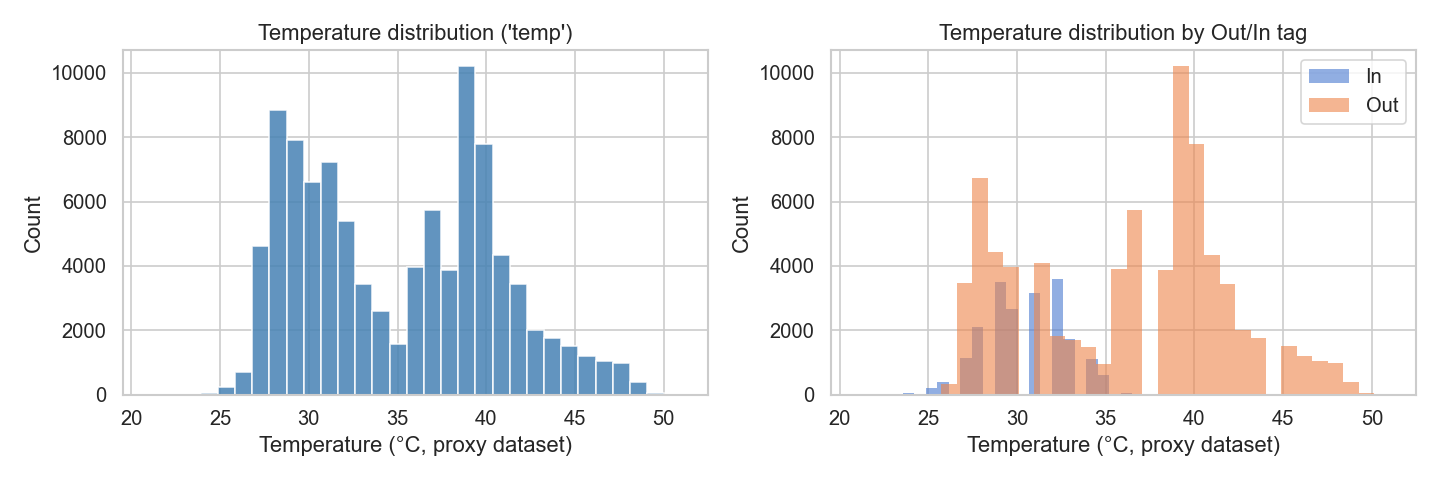
\includegraphics[width=0.95\textwidth]{figures/fig_temperature_distribution.png}\\[2pt]
            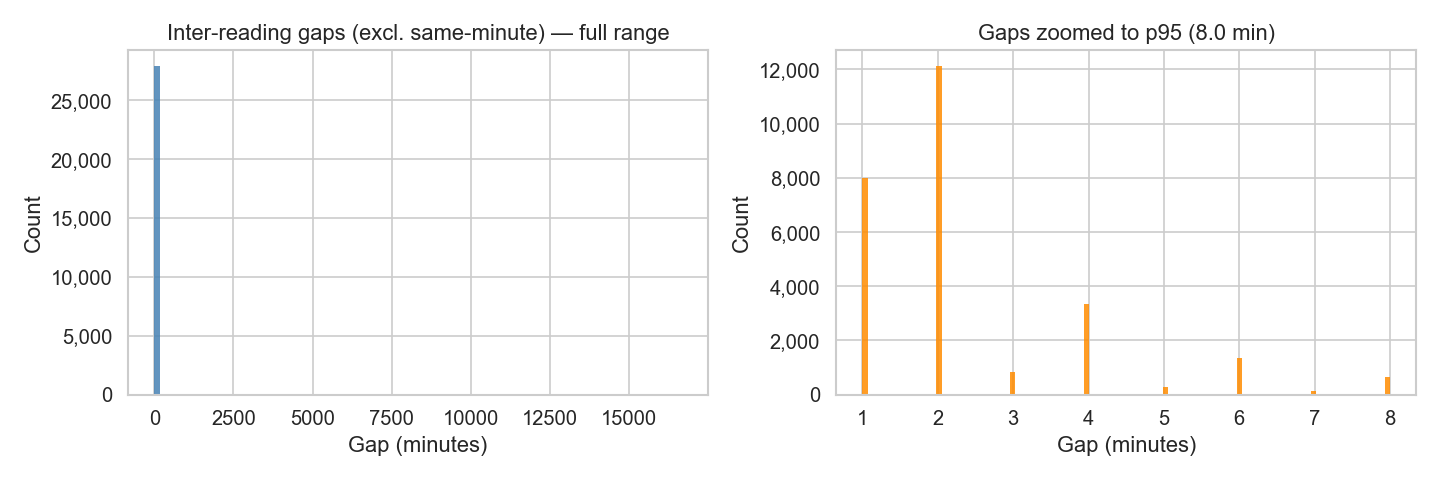
\includegraphics[width=0.95\textwidth]{figures/fig_sampling_intervals_corrected.png}
        \end{column}
    \end{columns}
    \note{We used a 97,000-reading real IoT dataset covering over 4 months. In real supply chains, sensor packets arrive irregularly due to network jitter and dropouts—our data reflects this with a high variance coefficient of 46.2. Importantly, we maintain complete academic honesty: we explicitly treat this as a structural proxy for sensor streaming, rather than fabricating claims of live pharmaceutical field testing.}
\end{frame}

% ------------------------------------------------------------------------------
% SLIDE 5: SYSTEM ARCHITECTURE & DIGITAL TWIN
% ------------------------------------------------------------------------------
\begin{frame}{System Architecture \& The Digital Twin}
    \begin{columns}[T]
        \begin{column}{0.48\textwidth}
            \begin{block}{SimPy Discrete-Event Digital Twin}
                \begin{itemize}\small
                    \item \textbf{Causal Ingestion:} Day-first parsing (\texttt{dayfirst=True}), trailing features (zero look-ahead leakage, D22).
                    \item \textbf{3-Stage Pipeline:} \texttt{Source} $\rightarrow$ \texttt{Transit} $\rightarrow$ \texttt{Destination} event-driven replay.
                    \item \textbf{Streaming Monitors:}
                    \begin{itemize}\footnotesize
                        \item \texttt{BaselineMonitor} ($2\sigma$ upper bound)
                        \item \texttt{IFMonitor} (Isolation Forest partition)
                        \item \texttt{LSTMMonitor} (Sliding-window MSE)
                    \end{itemize}
                    \item \textbf{Buffer Pre-Warming (D33):} Silently primes rolling buffers before visible playback, eliminating cold-start false negatives.
                \end{itemize}
            \end{block}
        \end{column}
        
        \begin{column}{0.50\textwidth}
            \centering
            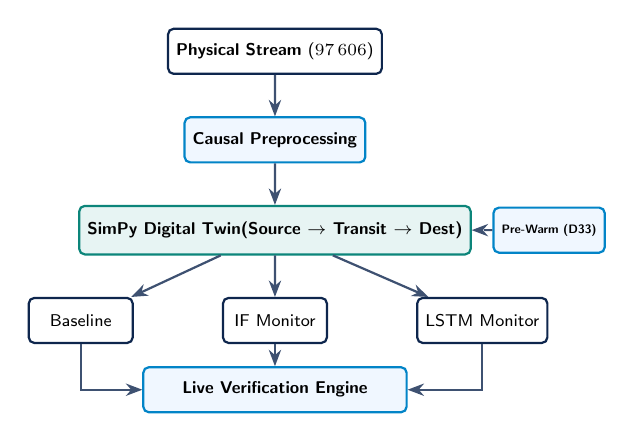
\begin{tikzpicture}[node distance=0.6cm and 0.4cm, scale=0.88, every node/.style={transform shape}]
                \node (raw) [sblock, minimum width=2.4cm] {\textbf{Physical Stream} (\num{97606})};
                \node (prep) [ablock, below=of raw, minimum width=2.4cm] {\textbf{Causal Preprocessing}};
                \node (simpy) [tblock, below=of prep, minimum width=2.8cm] {\textbf{SimPy Digital Twin}\\(Source $\rightarrow$ Transit $\rightarrow$ Dest)};
                \node (prew) [ablock, right=0.3cm of simpy, font=\tiny\sffamily\bfseries] {Pre-Warm (D33)};
                
                \node (mon_b) [sblock, below left=0.6cm and -0.8cm of simpy, minimum width=1.5cm] {Baseline};
                \node (mon_if) [sblock, below=0.6cm of simpy, minimum width=1.5cm] {IF Monitor};
                \node (mon_l) [sblock, below right=0.6cm and -0.8cm of simpy, minimum width=1.5cm] {LSTM Monitor};
                
                \node (eval) [ablock, below=1.6cm of simpy, minimum width=3.8cm] {\textbf{Live Verification Engine}};
                
                \draw [sarrow] (raw) -- (prep);
                \draw [sarrow] (prep) -- (simpy);
                \draw [sarrow, dashed] (prew) -- (simpy);
                \draw [sarrow] (simpy) -- (mon_b);
                \draw [sarrow] (simpy) -- (mon_if);
                \draw [sarrow] (simpy) -- (mon_l);
                \draw [sarrow] (mon_b) |- (eval);
                \draw [sarrow] (mon_if) -- (eval);
                \draw [sarrow] (mon_l) |- (eval);
            \end{tikzpicture}
        \end{column}
    \end{columns}
    \note{Our architecture consists of three stages: data ingestion, machine learning detectors, and an event-driven SimPy digital twin modeling Source, Transit, and Destination. When a telemetry event reaches Destination, our three monitors score it in real time. We implemented silent buffer pre-warming so the rolling buffers have history, eliminating cold-start errors.}
\end{frame}

% ------------------------------------------------------------------------------
% SLIDE 6: EXPERIMENTAL SETUP & ANOMALY PROTOCOL
% ------------------------------------------------------------------------------
\begin{frame}{Experimental Setup \& Anomaly Protocol}
    \begin{columns}[T]
        \begin{column}{0.48\textwidth}
            \begin{block}{Controlled Synthetic Injections (Seed 42)}
                \begin{itemize}\small
                    \item \textbf{30 Injections (15 Out / 15 In):}
                    \begin{itemize}\footnotesize
                        \item \textbf{Step Spikes (10):} $+5^\circ\text{C}$ to $+15^\circ\text{C}$ jumps.
                        \item \textbf{Linear Drifts (10):} $+0.05^\circ\text{C}$ to $+0.25^\circ\text{C}$/min.
                        \item \textbf{Sensor Flatlines (10):} Zero variance freeze.
                    \end{itemize}
                    \item \textbf{Chronological Split:} 70\% Train / 30\% Test (Cutoff: \texttt{2018-10-29 11:10:48}).
                    \item \textbf{Out-of-Sample Discipline:} All headline metrics restricted strictly to the \textbf{6 untouched test injections}.
                    \item \textbf{Lead Time Formula:}
                    $$\Delta t_{\text{lead}} = t_{\text{irreversibility}} - t_{\text{alarm}}$$
                \end{itemize}
            \end{block}
        \end{column}
        
        \begin{column}{0.50\textwidth}
            \centering
            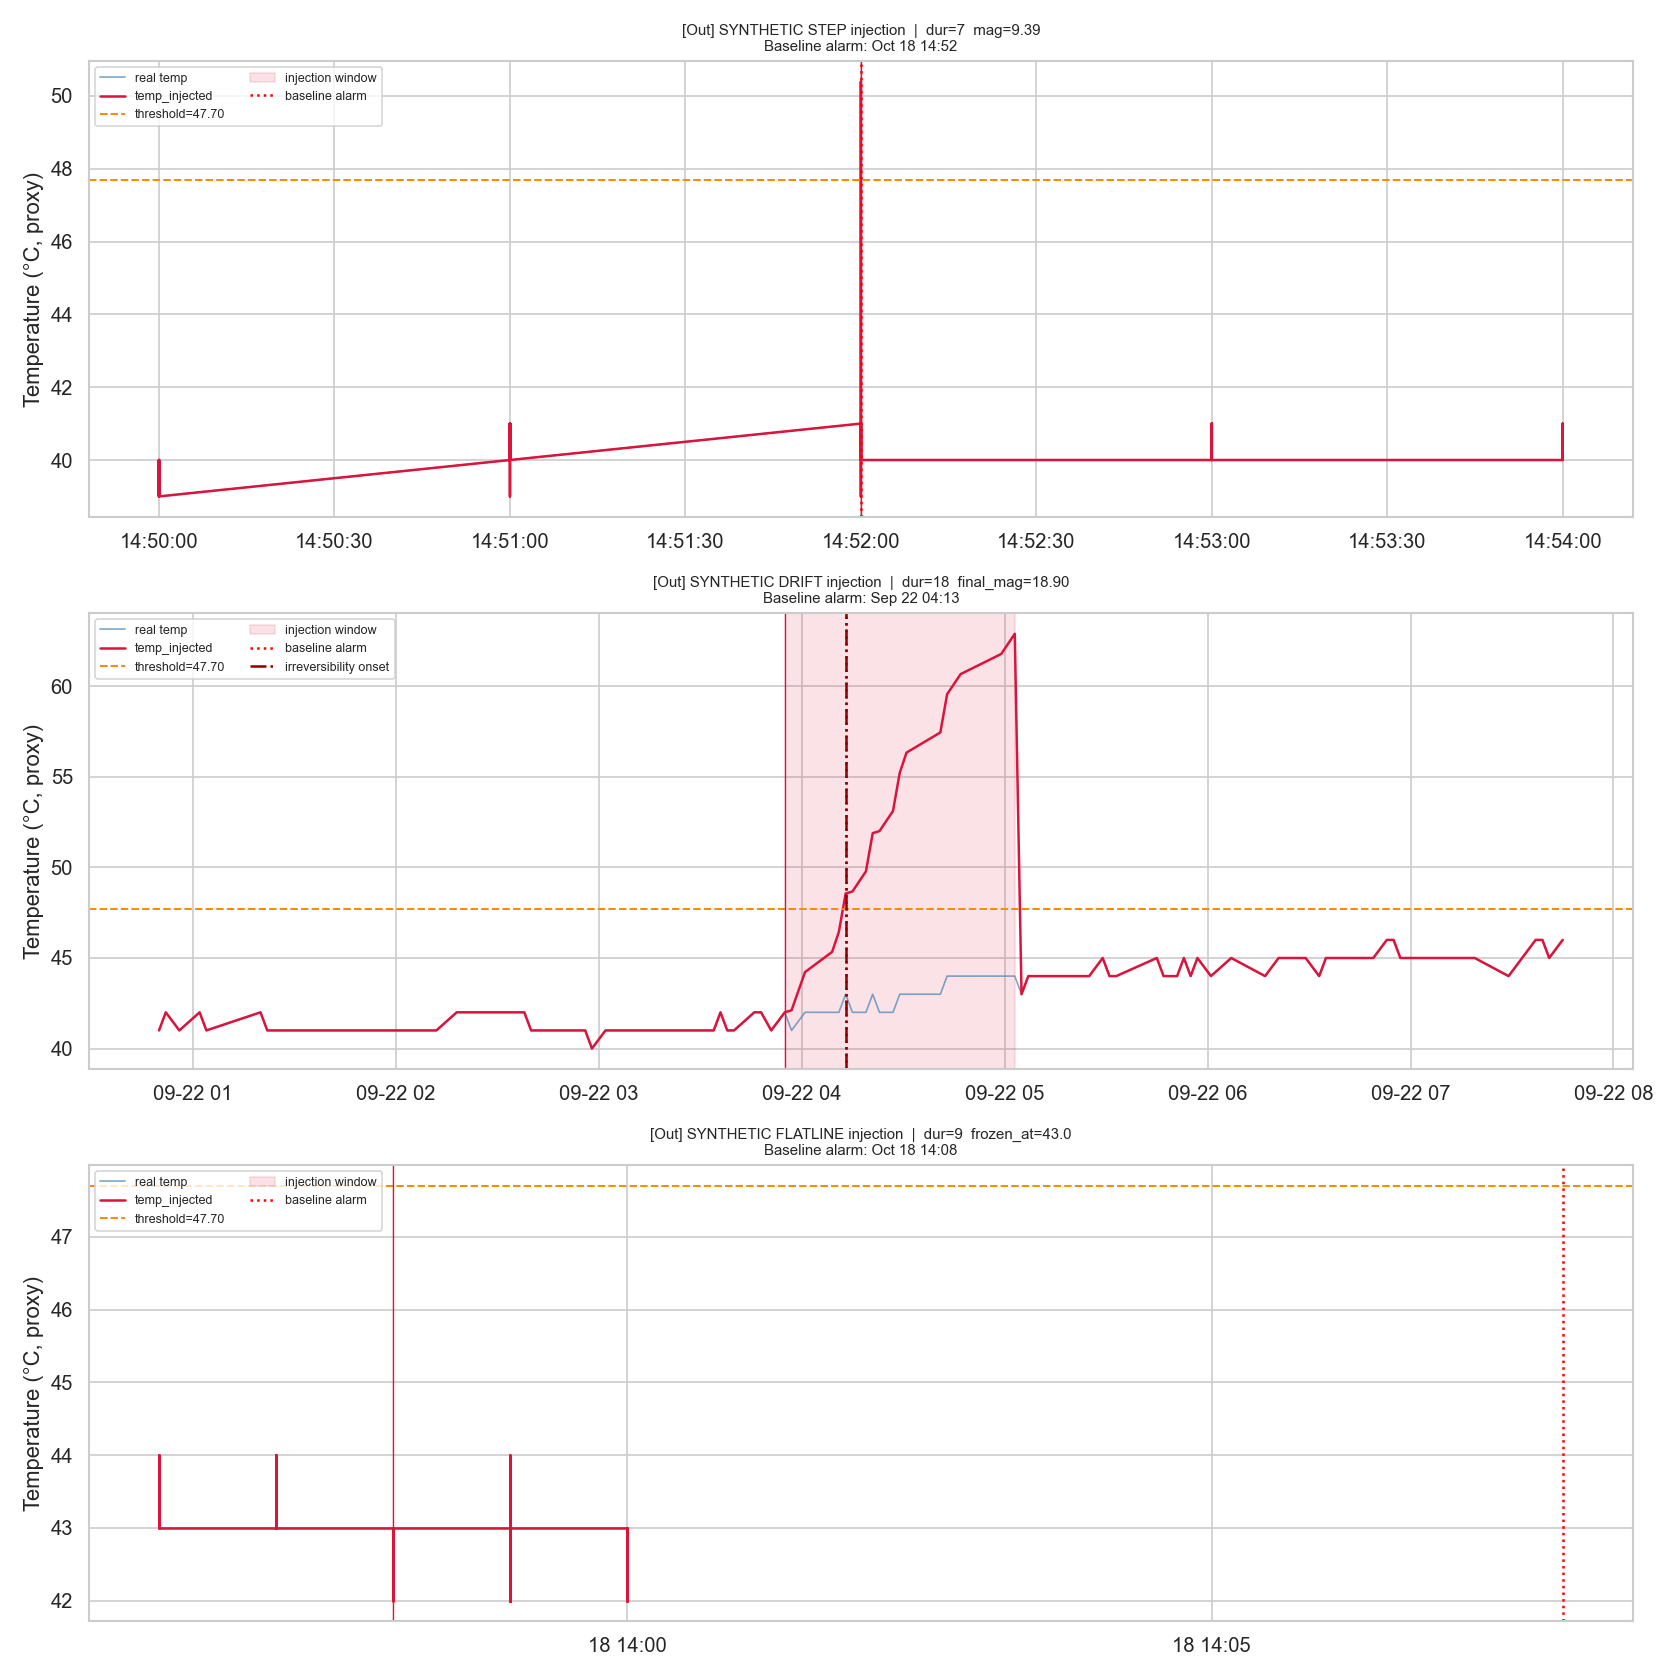
\includegraphics[width=\textwidth]{figures/fig_injection_examples.png}
        \end{column}
    \end{columns}
    \note{To test the system rigorously, we injected 30 controlled synthetic disruptions representing real failure modes: abrupt steps, gradual drifts, and flatlines. We enforced a strict chronological 70/30 train/test split. To ensure scientific validity, all our performance benchmarks are evaluated solely on the 6 untouched test-set injections.}
\end{frame}

% ------------------------------------------------------------------------------
% SLIDE 7: CORE RESULT 1 — EARLY-WARNING LEAD TIMES
% ------------------------------------------------------------------------------
\begin{frame}{Core Result 1: Early-Warning Lead Times (Test Split)}
    \begin{columns}[T]
        \begin{column}{0.55\textwidth}
            \centering
            \scriptsize
            \renewcommand{\arraystretch}{1.15}
            \begin{tabularx}{\textwidth}{L{2.0cm} C{0.8cm} C{1.2cm} C{1.3cm} C{1.3cm}}
                \toprule
                \rowcolor{NavyBlue}
                \textbf{\textcolor{white}{Injection ID}} & \textbf{\textcolor{white}{Type}} & \textbf{\textcolor{white}{Baseline}} & \textbf{\textcolor{white}{IF Lead Time}} & \textbf{\textcolor{white}{LSTM Lead}} \\
                \midrule
                \texttt{out\_step\_001}    & Step     & 0.0 min & 0.0 min & 0.0 min \\
                \texttt{out\_drift\_009}   & Drift    & 0.0 min & \textbf{\textcolor{EmeraldGreen}{+64.0 min}} & \textbf{\textcolor{CrimsonRed}{-14.0 min}} \\
                \texttt{out\_flatline\_012}& Flatline & Missed  & \textcolor{EmeraldGreen}{Detected} & \textcolor{EmeraldGreen}{Detected} \\
                \texttt{out\_flatline\_013}& Flatline & Missed  & \textcolor{EmeraldGreen}{Detected} & \textcolor{CrimsonRed}{Missed} \\
                \texttt{in\_step\_018}     & Step     & 0.0 min & 0.0 min & 0.0 min \\
                \texttt{in\_drift\_023}    & Drift    & 0.0 min & \textbf{\textcolor{EmeraldGreen}{+11.0 min}} & 0.0 min \\
                \bottomrule
            \end{tabularx}
            \vspace{6pt}
            \begin{block}{Key Findings}
                \footnotesize
                $\bullet$ \textbf{Drift Success:} IF flags subtle ramp-up \textbf{64 min} (\texttt{Out}) and \textbf{11 min} (\texttt{In}) early.\\
                $\bullet$ \textbf{Step Synchrony:} All detectors fire at onset (0.0 min lead time).\\
                $\bullet$ \textbf{LSTM Lag:} Delayed by 14 min on Out drift due to error adaptation.
            \end{block}
        \end{column}
        
        \begin{column}{0.43\textwidth}
            \centering
            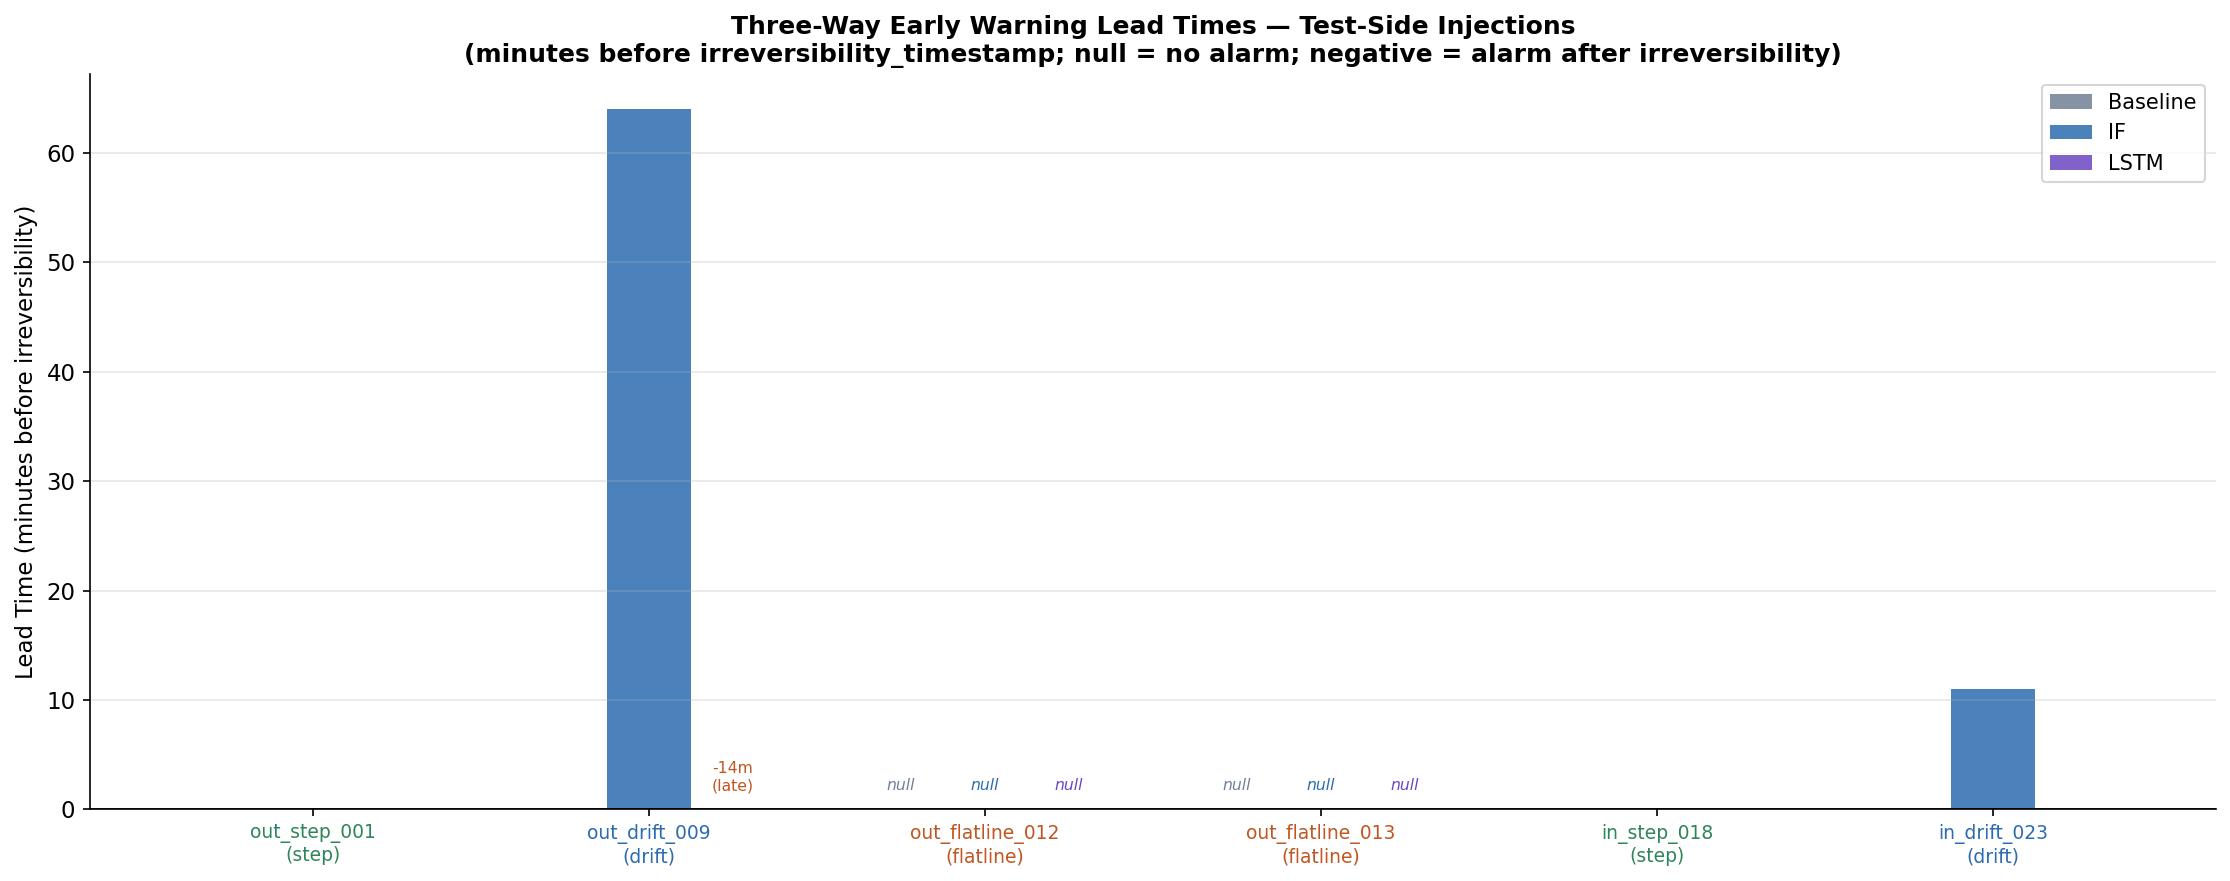
\includegraphics[width=\textwidth]{figures/fig_m4b_three_way_lead_times.png}
        \end{column}
    \end{columns}
    \note{Here is our primary research finding: On gradual drift disruptions—which represent slow compressor failures—Isolation Forest wins decisively, providing an early warning 64 minutes ahead on Out and 11 minutes ahead on In. On abrupt step breaches, all detectors trigger concurrently at 0 minutes. And for sensor flatlines, the traditional threshold completely fails to fire, while Isolation Forest catches both.}
\end{frame}

% ------------------------------------------------------------------------------
% SLIDE 8: CORE RESULT 2 — CLASSIFICATION TRADE-OFFS
% ------------------------------------------------------------------------------
\begin{frame}{Core Result 2: Classification Trade-Offs (D35 Data)}
    \begin{columns}[T]
        \begin{column}{0.48\textwidth}
            \begin{block}{Isolation Forest — High-Recall Tripwire}
                \begin{itemize}\footnotesize
                    \item \textbf{Recall:} 80.0\% (\texttt{Out}), 91.3\% (\texttt{In}).
                    \item \textbf{Trade-off:} High FPR (45.6\% \texttt{Out}, 27.0\% \texttt{In}).
                    \item \textbf{Role:} Aggressive frontline alarm to prevent missed excursions.
                \end{itemize}
            \end{block}
            
            \begin{exampleblock}{LSTM-Autoencoder — Precision Verifier}
                \begin{itemize}\footnotesize
                    \item \textbf{In Series:} Precision 13.11\%, FPR 2.85\%, AUC-PR 0.3852.
                    \item \textbf{Trade-off:} Lower recall on Out series (20.0\%).
                    \item \textbf{Role:} Conservative secondary verifier to reduce alarm fatigue.
                \end{itemize}
            \end{exampleblock}
            \tiny *Extreme anomaly rarity (~0.5\%) naturally caps absolute F1; early warning runway ($\Delta t_{\text{lead}}$) is the primary operational metric.
        \end{column}
        
        \begin{column}{0.50\textwidth}
            \centering
            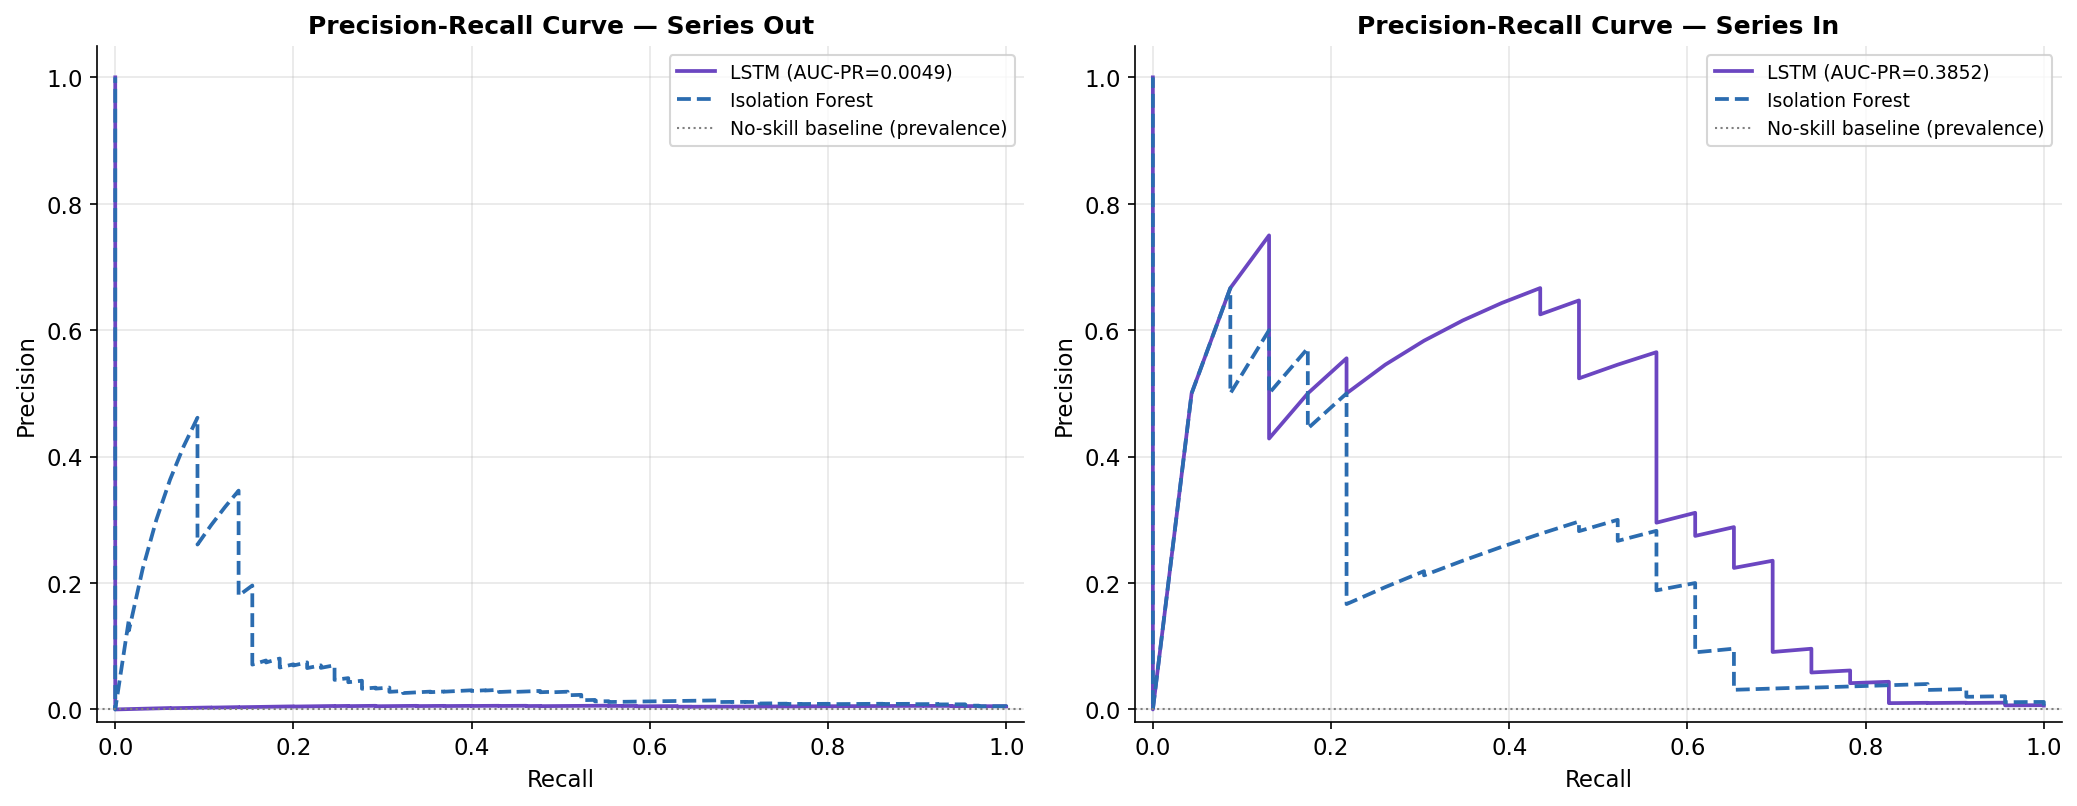
\includegraphics[width=\textwidth]{figures/fig_m4b_pr_curves.png}
        \end{column}
    \end{columns}
    \note{When looking at point-wise metrics, we see a classic engineering trade-off: Isolation Forest acts as an aggressive tripwire with high recall over 80–90%, but at the cost of a higher false-alarm rate. In contrast, the LSTM is highly conservative on the In series with a 2.85% false-positive rate and higher precision. Neither detector universally dominates, showing why hybrid architectures are valuable.}
\end{frame}

% ------------------------------------------------------------------------------
% SLIDE 9: DIGITAL TWIN PARITY & LIVE DASHBOARD
% ------------------------------------------------------------------------------
\begin{frame}{Digital Twin Parity \& Interactive Live Dashboard}
    \begin{columns}[T]
        \begin{column}{0.48\textwidth}
            \begin{block}{Simulation Fidelity Verification}
                \begin{itemize}\small
                    \item \textbf{100\% Bit-for-Bit Parity:} SimPy replayed \num{97603} events in \SI{6.03}{\second} ($>1.9\text{M}\times$ real-time speedup) with \textbf{\SI{0.00}{\second}} timing divergence.
                    \item \textbf{Zero Mismatches:} Across 30 injections $\times$ 3 monitors, all 42 applicable test evaluations matched batch outputs identically.
                    \item \textbf{Automated Test Suite:} Automated regression tests (\texttt{test\_d33\_prewarm.py}) pass in 15.3 s.
                \end{itemize}
            \end{block}
        \end{column}
        
        \begin{column}{0.50\textwidth}
            \begin{exampleblock}{Deployed Streamlit Cloud UI}
                \begin{itemize}\small
                    \item \textbf{Public Link:}\\
                    \href{https://coldchain-ews-twin.streamlit.app/}{\texttt{coldchain-ews-twin.streamlit.app}}
                    \item \textbf{Guided Tour Mode:}\\
                    4-step curated walkthrough for viva demonstrations.
                    \item \textbf{Free Explore Mode:}\\
                    Interactive inspection of all 30 injections.
                    \item \textbf{Single Source of Truth:}\\
                    Captions dynamically interpolated from verified CSVs (D34); zero hardcoded UI metrics.
                \end{itemize}
            \end{exampleblock}
        \end{column}
    \end{columns}
    \note{To prove that embedding these models in a simulation loop doesn't cause silent discrepancies, our automated cross-check report achieved a 100% exact match across all 42 applicable comparisons. Furthermore, the entire system is deployed live on Streamlit Cloud, featuring an interactive Guided Tour designed specifically for viva examination walkthroughs.}
\end{frame}

% ------------------------------------------------------------------------------
% SLIDE 10: CONCLUSION & CORPORATE ENTREPRENEURSHIP RELEVANCE
% ------------------------------------------------------------------------------
\begin{frame}{Conclusion \& Corporate Entrepreneurship Relevance}
    \begin{block}{Key Technical \& Corporate Takeaways}
        \begin{enumerate}\small
            \item \textbf{Evidence-First Engineering:} Transparent reporting of real trade-offs: We documented where deep learning lagged on drift and where classical ML excelled, avoiding superficial 99\% accuracy claims.
            \item \textbf{Disciplined Auditability:} Maintained an append-only Architectural Decision Log (35 formal entries D1--D35), catching 4 critical bugs before they could bias evaluation.
            \item \textbf{Technology Adoption Strategy:} Proved that classical ML (Isolation Forest) delivers high operational runway (+64 min lead time) at low compute overhead for edge streams.
            \item \textbf{Complete Deliverable Portfolio:} Verified SimPy twin, pre-trained weights, live web dashboard, and 12-chapter LaTeX report.
        \end{enumerate}
    \end{block}
    \vspace{4pt}
    \begin{center}
        \textbf{\textcolor{NavyBlue}{\Large Thank you! Open for Questions \& Live Demo}}\\[3pt]
        \small\texttt{coldchain-ews-twin.streamlit.app}
    \end{center}
    \note{To conclude: this project bridges machine learning, discrete-event digital twins, and disciplined corporate entrepreneurship. We did not cherry-pick our data or claim artificial perfection—we demonstrated exactly where classical ML provides real operational runway, where deep learning lags, and how an organization can rigorously evaluate technology under uncertainty. Thank you, and I look forward to your questions.}
\end{frame}

\end{document}
